% !TeX program = pdflatex
\documentclass[tikz,border=8pt]{standalone}
\usepackage{tikz}
\usetikzlibrary{calc,intersections,positioning}
\definecolor{FigureBlue}{HTML}{2563EB}
\definecolor{FigureOrange}{HTML}{EA580C}
\begin{document}
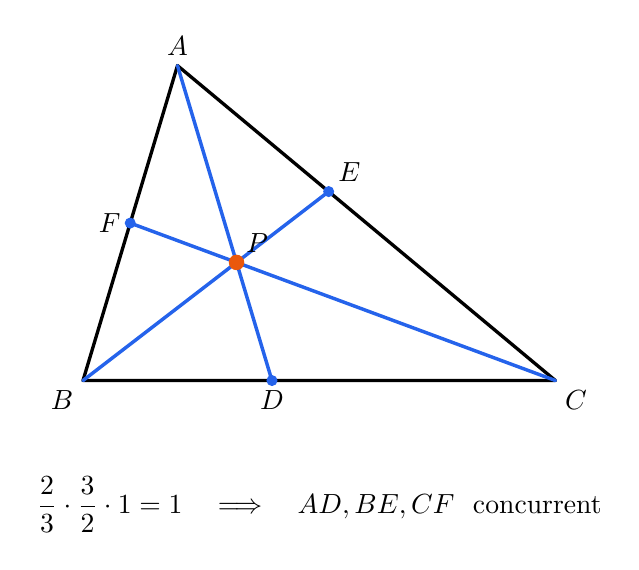
\begin{tikzpicture}[line cap=round,line join=round]
  \coordinate (A) at (1.2,4);\coordinate (B) at (0,0);\coordinate (C) at (6,0);
  \coordinate (D) at ($(B)!.4!(C)$);
  \coordinate (E) at ($(C)!.6!(A)$);
  \coordinate (F) at ($(A)!.5!(B)$);
  \path[name path=AD] (A)--(D);\path[name path=BE] (B)--(E);
  \path[name intersections={of=AD and BE,by=P}];
  \draw[line width=1.2pt] (A)--(B)--(C)--cycle;
  \draw[FigureBlue,line width=1.25pt] (A)--(D) (B)--(E) (C)--(F);
  \foreach \P in {D,E,F}{\fill[FigureBlue] (\P) circle (2pt);}
  \fill[FigureOrange] (P) circle (2.8pt);
  \node[above] at (A) {$A$};\node[below left] at (B) {$B$};\node[below right] at (C) {$C$};
  \node[below] at (D) {$D$};\node[above right] at (E) {$E$};\node[left] at (F) {$F$};\node[above right] at (P) {$P$};
  \node[below=11mm] at ($(B)!.5!(C)$) {$\displaystyle\frac23\cdot\frac32\cdot1=1\quad\Longrightarrow\quad AD,BE,CF\ \hbox{ concurrent}$};
\end{tikzpicture}
\end{document}
